% ==============================================
\section{Introduction}
\label{sec:intro}
% ==============================================

\begin{figure}
\centering
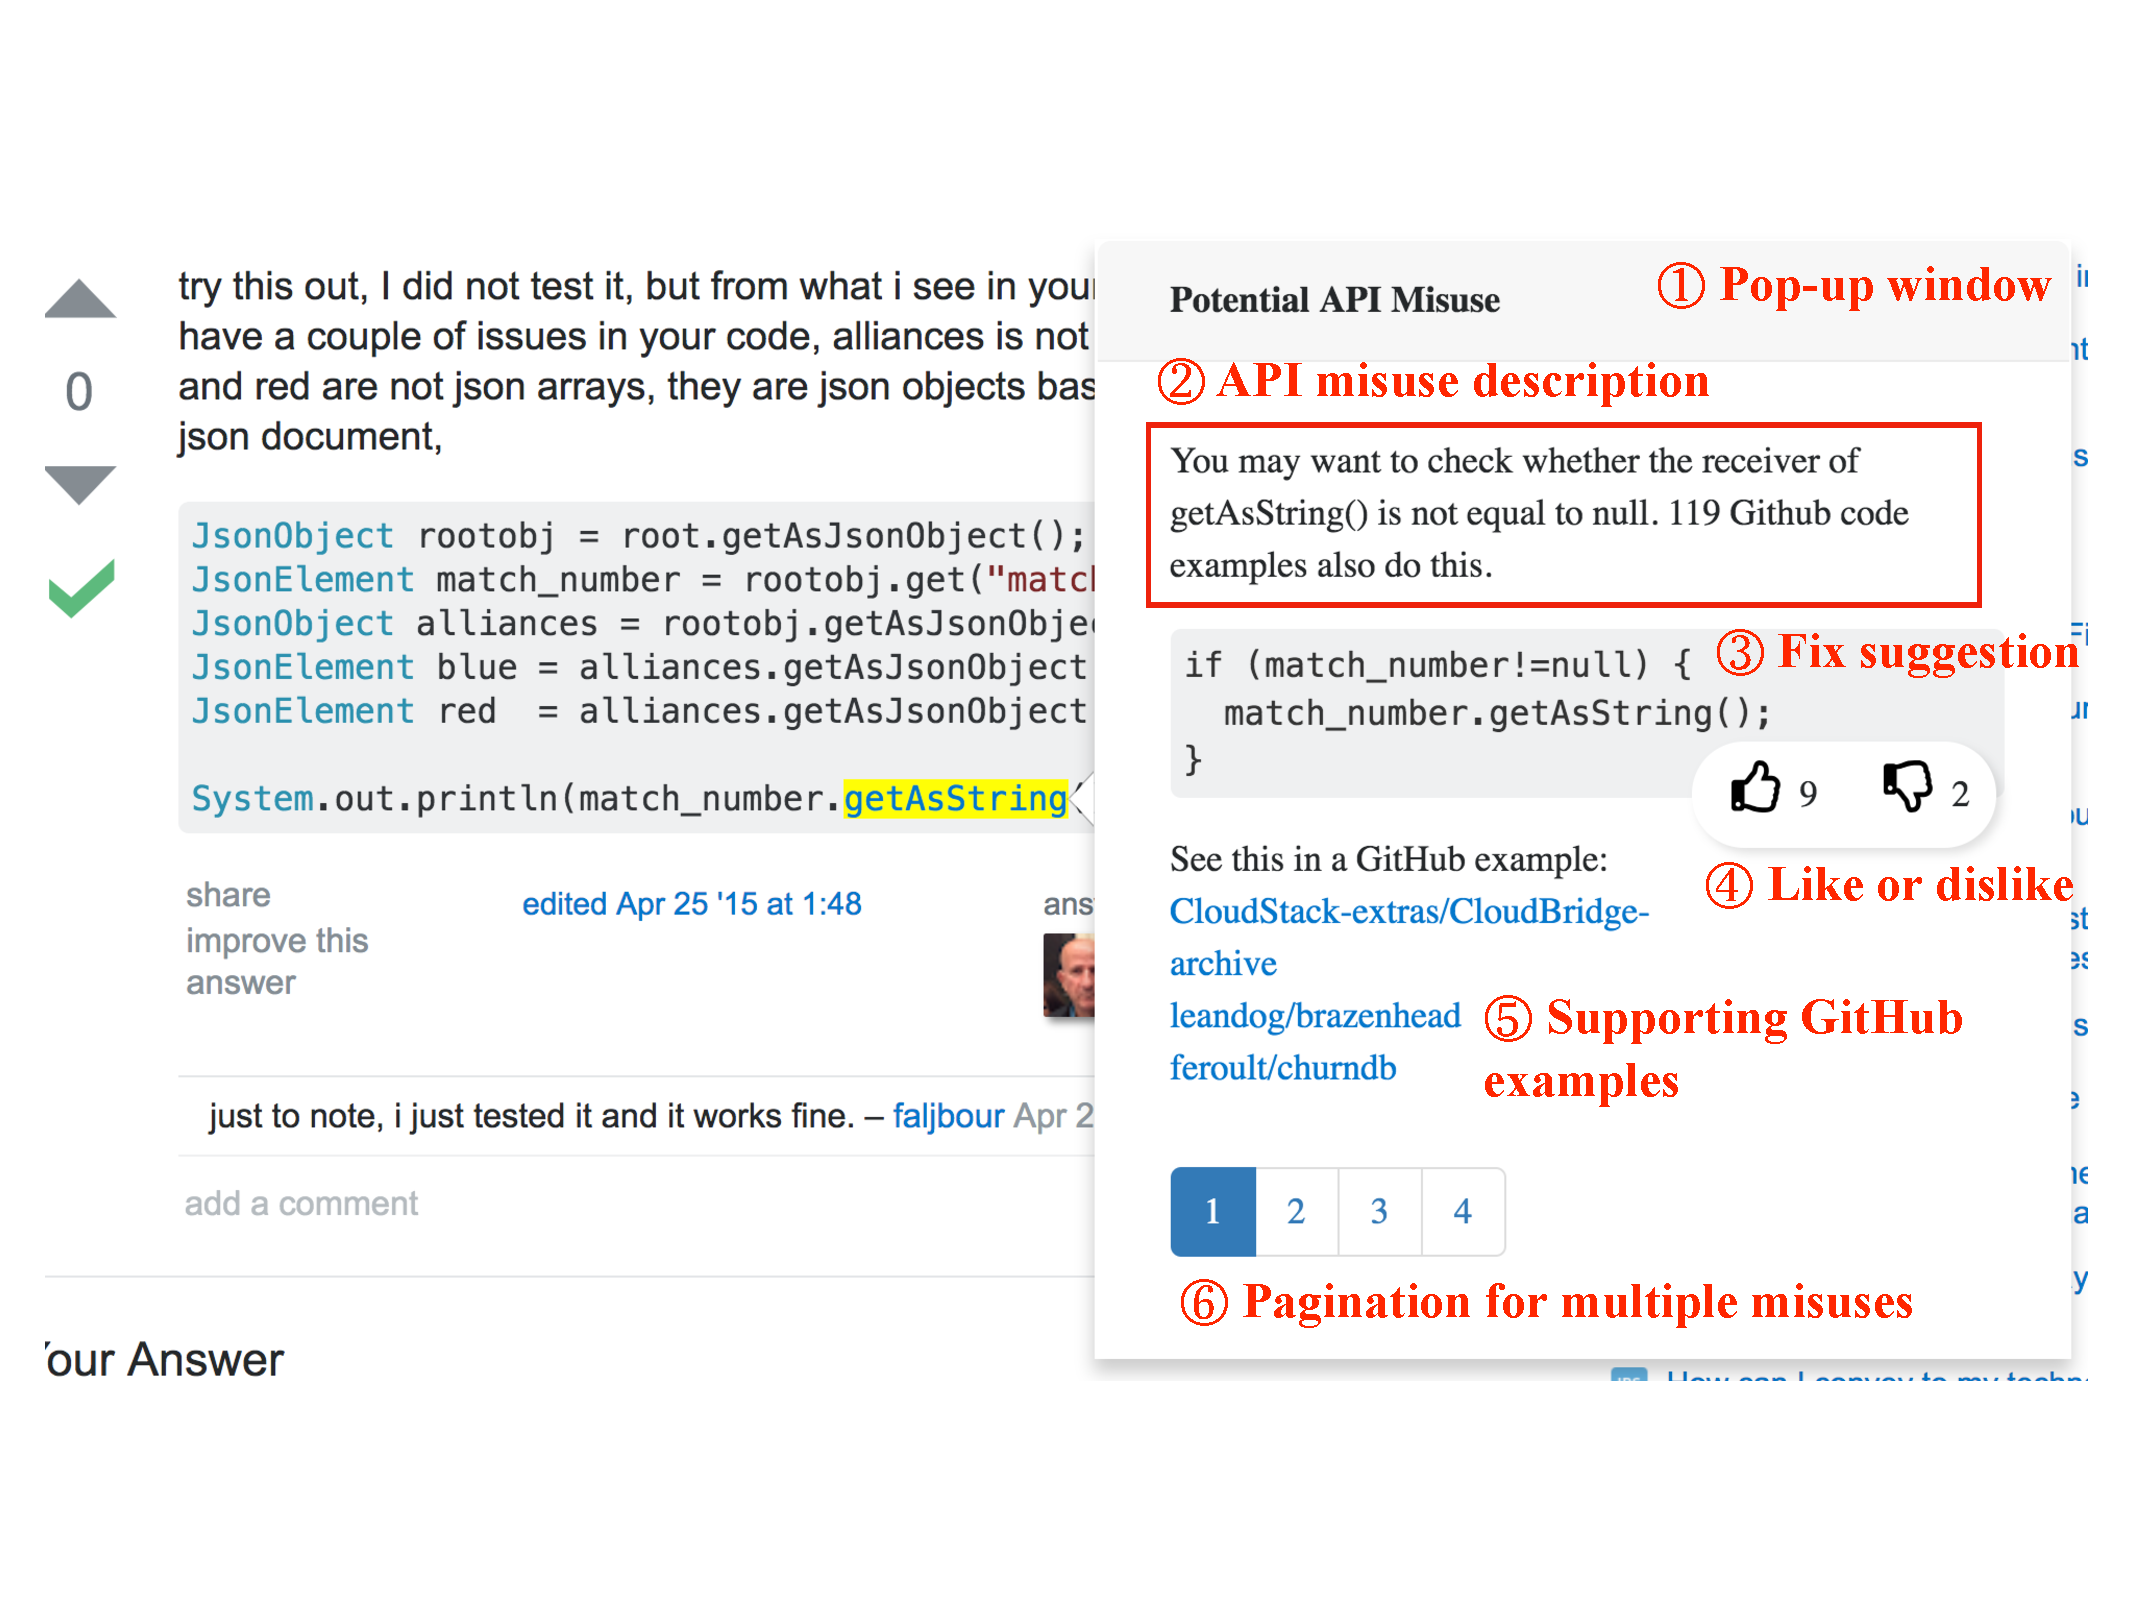
\includegraphics[width=0.5\textwidth]{examplecheck-screenshot.pdf}
  \caption{The {\tool} Chrome extension that augments Stack Overflow with API misuse warnings. The pop-up window alerts that {\ttt match\_number} can be {\ttt null} if the requested {\ttt JSON} attribute does not exist and will crash the program by throwing {\ttt NullPointerException} when {\ttt getAsString} is called on it.}
  \label{fig:screenshot}
  \vspace{-0.1in}
\end{figure}

% Problem
Programmers often search for online code examples to learn new APIs. A case study at Google shows that developers issue an average of 12 code search queries per weekday~\cite{sadowski2015developers}. Stack Overflow (SO) is a popular Q\&A website that programmers often resort to. As of July 2017, Stack Overflow has accumulated more than 22 million answers, many of which contain code snippets for specific programming questions. However, SO snippets are not always complete or reliable, which can be misleading and sometimes harmful when programmers follow them {\em as-is} during software development. For example, Fischer et al.~find that 29\% of security-related code snippets in Stack Overflow are insecure and might affect over 1 million Android apps in Google play~\cite{fischer2017stack}. 

% Solution
This tool demonstration paper builds on the API usage mining and API misuse detection technique described in our ICSE 2018 paper~\cite{zhang2018code}. Our insight is that common API usage inferred from a large corpus of 380K GitHub projects may represent a desirable pattern that a programmer can use to examine and enhance SO code snippets. Mined API usage patterns abstract away syntactic details such as variable names, but retain the temporal ordering, control structures, and guard conditions of API calls. 

\begin{figure*}[!th]
\centering
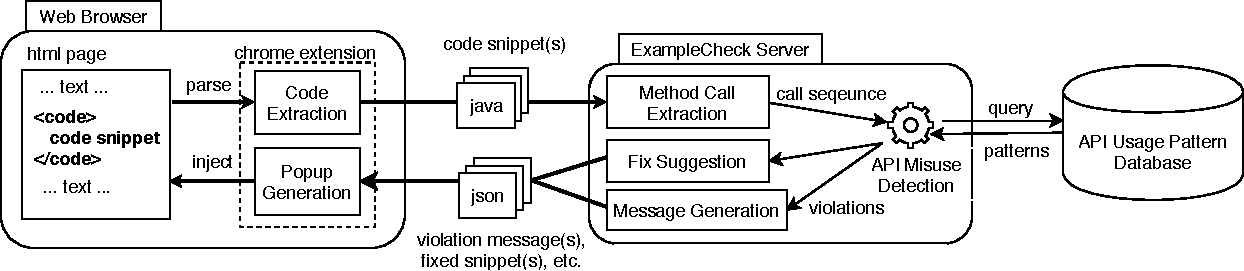
\includegraphics[width=0.85\textwidth]{examplecheck-extension.pdf}
\caption{An overview of {\tool}'s architecture}
\label{fig:arch}
\end{figure*}

This paper, in particular, focuses on the tool features and implementation details of a Chrome extension, called {\tool} that informs programmers about API usage violations in SO posts. Figure~\ref{fig:screenshot} shows a screenshot of {\tool}. Given a SO post, {\tool} first extracts the sequence of API calls with corresponding control constructs and guard conditions. {\tool} then contrasts the call sequence against the common API usage patterns mined from GitHub. To help users understand a detected violation, {\tool} generates a descriptive warning message and illustrates how to fix the violation with corresponding GitHub examples. Using common API usage patterns to detect violations may lead to false alarms, since these mined, common patterns do not necessarily represent correct API usage. To mitigate this issue, {\tool} allows users to upvote or downvote a reported violation based on its applicability and usefulness. 

The resulting data set of mined API usage patterns, detected violations in Stack Overflow, and our manual inspection result are publicly available at~{\small\url{http://web.cs.ucla.edu/~tianyi.zhang/examplecheck.html}}. The Chrome extension is available for download at Chrome Web Store~\cite{examplecheck}.

%A user of {\tool} would benefit from the addition of concrete examples from the production code in GitHub, when inspecting or reusing code snippets in Stack Overflow. This will not only combat programming issues stemming from the use of incomplete or unreliable SO code snippets, but will also be an aid for users learning a new API. 

%A user of this tool would benefit from not needing to cross-reference multiple sites for proper API usage reference, and will be able to continue using Stack Overflow to learn APIs with the added advantage of seeing which usage patterns a post may have left out of its explanation. This could result in more complete, reliable code with minimal added time or effort on the part of the programmer.\todo{The description here does not sound very appealing. Can you rework this paragraph?} 

%input{fig_motiExample}
%\input{fig_UI}
